\chapter{PEMBIAYAAN KESEHATAN}
Pembiayaan kesehatan bertujuan untuk penyediaan pembiayaan kesehatan yang berkesinambungan dengan jumlah yang mencukupi, teralokasi secara adil, dan termanfaatkan. Pembiayaan kesehatan merupakan besarnya dana yang harus disediakan untuk menyelenggarakan dan atau memanfaatkan berbagai upaya kesehatan yang diperlukan oleh perorangan, keluarga, kelompok, dan masyarakarat.

Secara umum, sumber biaya kesehatan dapat dibedakan menjadi pembiayaan yang bersumber dari anggaran pemerintah dan pembiayaan yang bersumber dari masyarakat.

\section[PEMBIAYAAN OLEH MASYARAKAT]{PEMBIAYAAN KESEHATAN OLEH MASYARAKAT}
Pada saat ini berkembang berbagai upaya pembiayaan pelayanan kesehatan praupaya, antara lain Badan Penyelenggara Jaminanan Sosial Kesehatan (BKPJS Kesehatan) dan berbagai jasa asuransi kesehatan swasta. BPJS Kesehatan adalah Badan Hukum Publik yang bertanggung jawab langsung kepada Presiden dan memiliki tugas untuk menyelenggarakan Jaminan Kesehatan Nasional bagi seluruh rakyat Indonesia. Keanggotaan BPJS bersifat wajib bagi setiap warga negara Indonesia dan warga asing yang sudah bekerja di Indonesia selama minimal enam bulan. Setiap peserta BPJS akan ditarik iuran yang besarnya ditentukan kemudian, sesuai dengan tingkatan manfaat yang diinginkan.

Sejak tahun 2014, penyelenggaraan pelayanan kesehatan bagi masyarakat miskin meliputi pelayanan kesehatan dasar di Puskesmas dan jaringannya, serta upaya kesehatan rujukan di Rumah Sakit telah dialihkan ke pengelolaan oleh BPJS Kesehatan. Bagi warga miskin, iuran BPJS ditanggung pemerintah melalui program Penerima Bantuan Iuran (PBI) yang dananya bersumber dari APBN maupun APBD Provinsi/ Kabupaten/ Kota.

Cakupan jaminan kesehatan melalui BPJS Kesehatan di Kabupaten Belitung Timur pada tahun \tP adalah sebesar 98,04\% dari jumlah penduduk, di mana 62,79\%  dari jumlah penduduk adalah Penerima Bantuan Iuran (PBI) bersumber APBD dan APBN (\autoref{fig:Cakupan-BPJS}).
%Diperkirakan terdapat 5.075 penduduk dari total 125.598 penduduk yang masih belum mendapat perlindungan jaminan kesehatan (\autoref{fig:Cakupan-Jamkes}).

\begin{figure}[H]
    \centering{}
    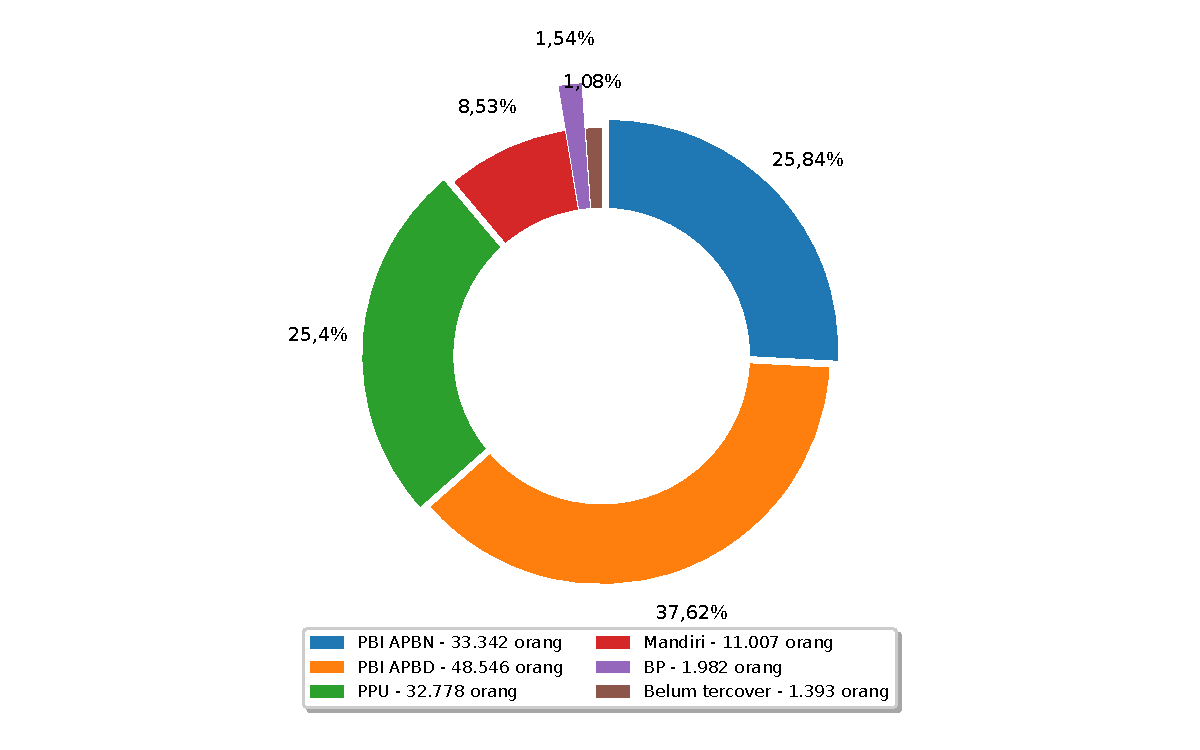
\includegraphics[width=0.9\textwidth]{bab_04/bab_04_01_jaminanKesehatan_a}
    \caption{Cakupan BPJS Kesehatan Kab. Belitung Timur Tahun \tP}
    \label{fig:Cakupan-BPJS}
\end{figure}

\begin{figure}[H]
    \centering{}
    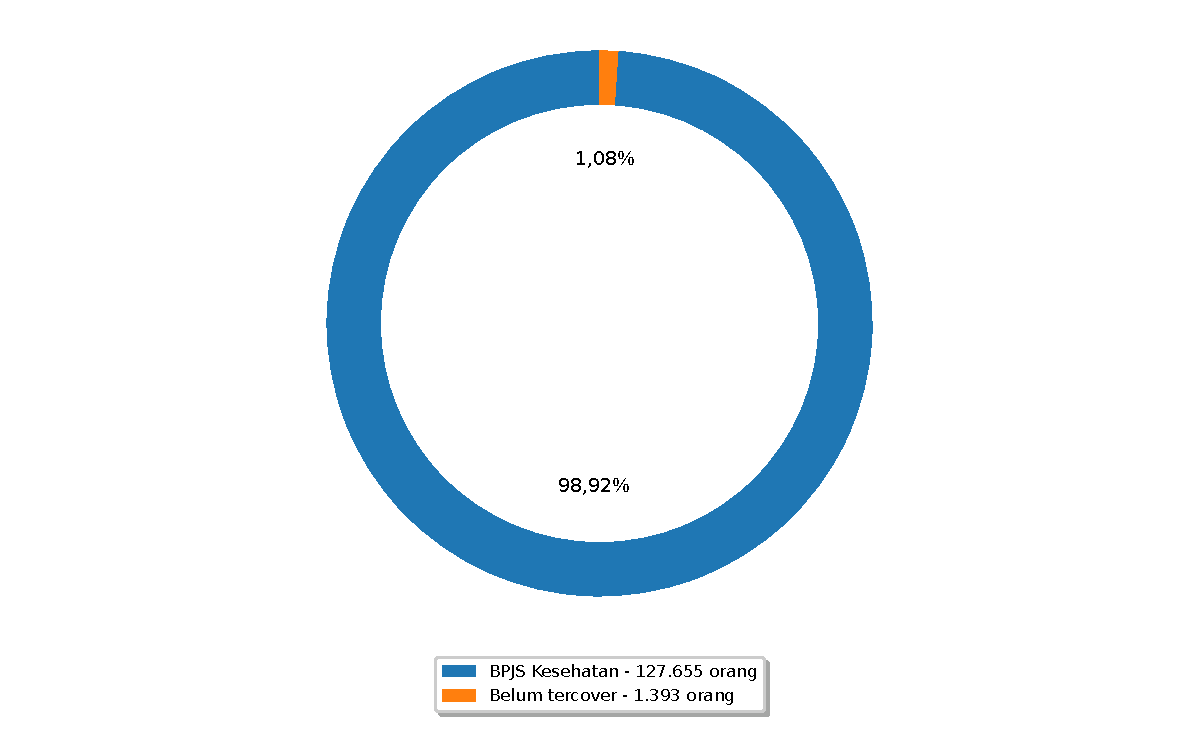
\includegraphics[width=0.9\textwidth]{bab_04/bab_04_01_jaminanKesehatan_b}
    \caption{Cakupan Jaminan Kesehatan Kab. Belitung Timur Tahun \tP}
    \label{fig:Cakupan-Jamkes}
\end{figure}

\section[PEMBIAYAAN OLEH PEMERINTAH]{PEMBIAYAAN KESEHATAN OLEH PEMERINTAH}
\subsection{Pembiayaan Melalui Anggaran Pendapatan dan Belanja Daerah}
Alokasi Anggaran Kesehatan di Kabupaten Belitung Timur pada tahun \tP melalui APBD Kabupaten Belitung Timur Tahun \tP (mencakup anggaran Dinas Kesehatan, UPTD Kesehatan dan RSUD Belitung Timur) adalah sebesar Rp 312.608.364.718. Nilai anggaran ini terdiri dari sumber APD murni sebesar Rp 295.065.063.220, Dana Alokasi Khusus (DAK) berupa DAK Fisik sebesar Rp 4.176.471.000 dan DAK Non-Fisik sebesar Rp 6.592.322.000. Selain itu terdapat anggaran belanja bersumber APBN berupa dana kapitasi sebesar Rp 6.740.864.498.

Porsi alokasi anggaran kesehatan adalah sebesar 33,94\% dari jumlah belanja APBD Kabupaten Belitung Timur Tahun \tP sebesar Rp 901.076.212.953. Sedangkan alokasi anggaran kesehatan per kapita adalah sebesar Rp 2.294.066,00 /kapita.

\begin{figure}[htb]
    \centering{}
    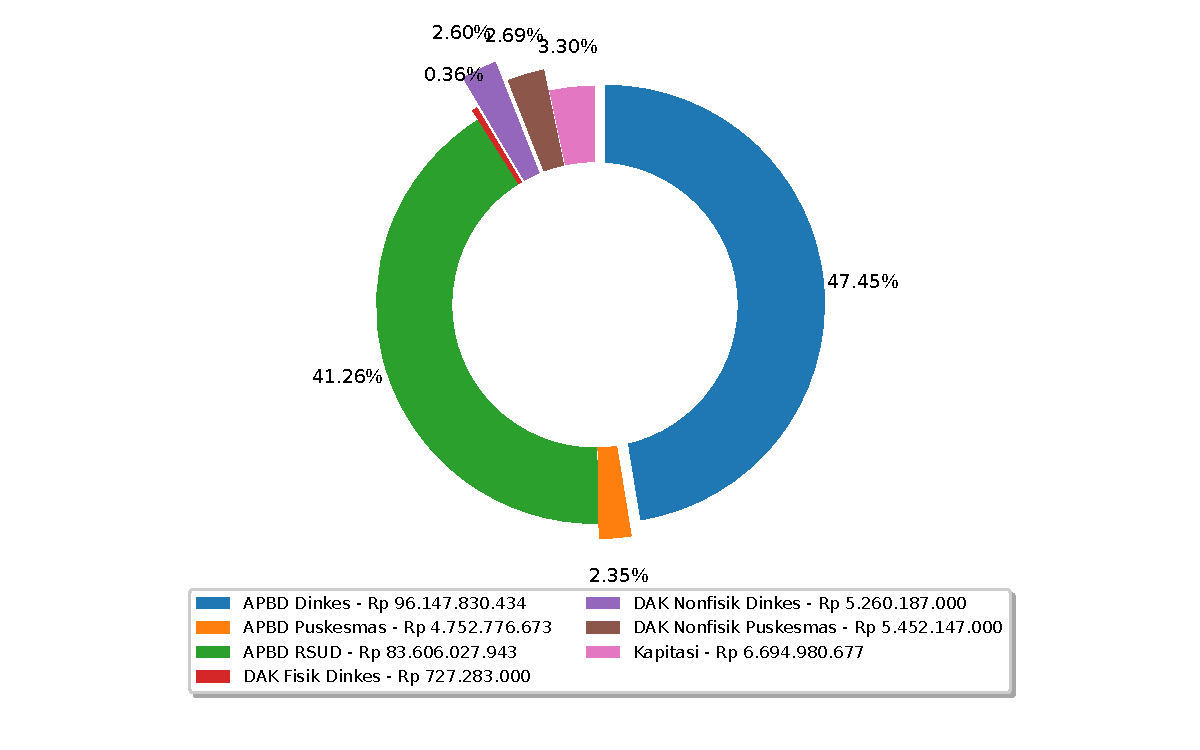
\includegraphics[width=0.9\textwidth]{bab_04/bab_04_03_anggaranKesehatan}
    \caption{Persentase Anggaran Kesehatan Kab. Belitung Timur Tahun \tP}
    \label{fig:Anggaran-Kesehatan}
\end{figure}

\subsection{Pembiayaan Jaminan Kesehatan Masyarakat Pada Anggaran DinkesPPKB}
Pembiayaan jaminan kesehatan masyarakat berupa iuran dan bantuan iuran jaminan kesehatan bagi peserta PBPU dan BP kelas 3 dianggarkan pada anggaran Dinas Kesehatan, Pengendalian Penduduk dan Keluarga Berencana Kabupaten Belitung Timur melalui Program Pemenuhan Upaya Kesehatan Perorangan Dan Upaya Kesehatan Masyarakat, Kegiatan Penyediaan Layanan Kesehatan untuk UKM dan UKP Rujukan Tingkat Daerah Kabupaten/Kota, Subkegiatan Pengelolaan Jaminan Kesehatan Masyarakat. Pada tahun \tP belanja iuran jaminan tersebut dianggarkan sebesar Rp 20.702.382.400 atau sebesar 18,49\% dari anggaran DinkesPPKB Kabupaten Belitung Timur.

\begin{figure}[htb]
	\centering{}
	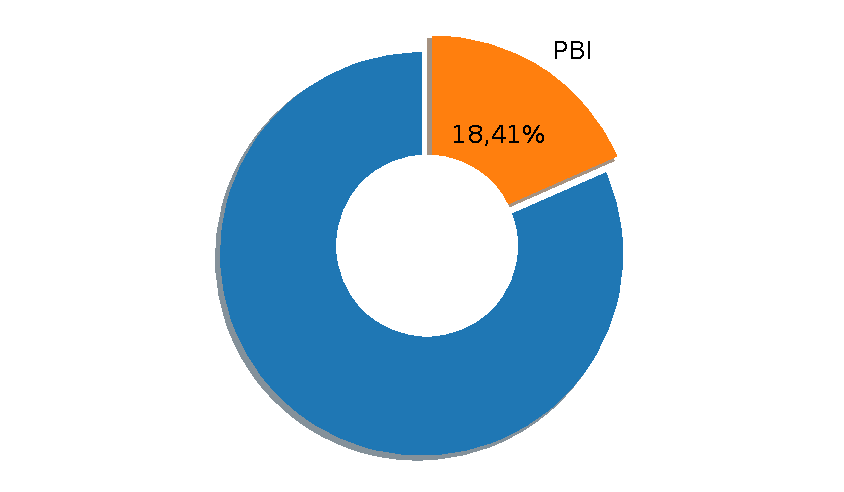
\includegraphics[width=0.9\textwidth]{bab_04/bab_04_04_proporsiPBI}
	\caption{Proporsi PBI terhadap Anggaran DKPPKB Kab. Belitung Timur Tahun \tP}
	\label{fig:Proporsi-PBI}
\end{figure}
